\documentclass[11pt]{article}
\usepackage{amsmath,tikz}

\usetikzlibrary{arrows}

\title{Bless, a pager\footnote{not like less}}
\author{void-}

\begin{document}
\maketitle
\section*{Overview}
\subsection*{Goal}
The Sender wishes to send a message to (i.e. page) the Receiver in real time.
The location of the Receiver should be private and the confidentiality,
integrity, and authenticity of the message should be preserved. The Sender must
also be approved to send messages to the Receiver, that is to say, not just
anyone can send a message to the Receiver. The system is designed to provide a
loose sense of the privacy of the Receiver's location when behind a NAT.

\section*{An illustration}
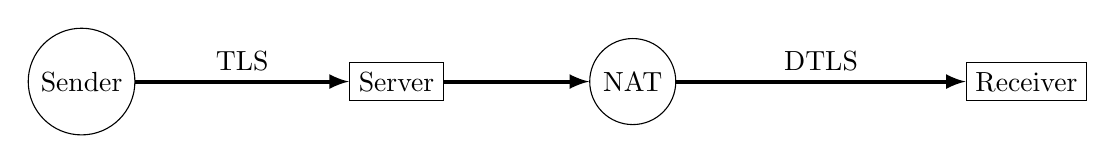
\begin{tikzpicture}
\node[draw, circle] at (0,0) (sender) {Sender};
\node[draw, rectangle] at (4,0) (server) {Server};
\node[draw, circle] at (7,0) (nat) {NAT};
\node[draw, rectangle] at (12,0) (receiver) {Receiver};

\draw[arrows={-latex}, line width=.5mm]
  (sender) to node[above] {TLS} (server);
\draw[arrows={-latex}, line width=.5mm] (server) to (nat);
\draw[arrows={-latex}, line width=.5mm] (nat) to node[above] {DTLS}
  (receiver);
%\draw[arrows={-latex}, line width=.5mm]
%  (anonymizer) to node[above] {message channel} (receiver);
\end{tikzpicture}

\section*{How it works}
Alice is the Sender, Bob the Receiver. Alice wants to send a message to Bob
while Bob is in an undisclosed location with internet access. Prior to this,
Alice and Bob exchanged public keys and the routing address of Bob's server(the
Server).

Bob, somewhere in the world, is connected to a NATed wifi router with his
device. Bob initially makes a DTLS connection to his own Server. This
bootstraps what is called the ``message channel''. This creates a UDP hole
punch in the NAT to facilitate a push protocol between the Server and Bob.
The Server will send periodic, heartbeats over the message channel to keep the
hole punch active.

When Alice sends the Server a message, the Server will authenticate her and
forward the message onto Bob. If Bob changes his physical location in the
world, the DTLS packets sent by the Server will unknowingly go undelivered.

\subsection*{In More Details}
When Bob makes the initial DTLS connection to the Server he indeed reveals his
location. However, from this point onward, Bob never sends another packet; this
is allowed because DTLS uses UDP as the underlying protocol.

From the perspective of the Server and, in general, any third party observer,
there is no way to determine if a message is ever successfully delivered to
Bob. This ensures that at any point in time after his initial connection, it is
not possible to determine if Bob is still connected to the same NAT. How does
this work? This relies on the behaviour and the otherwise indifference of the
NAT Bob is behind.

First and foremost, this discussion considers a wifi router to operate as a
NAT. Wifi routers commonly use ARP to determine if one of its clients is still
connected. Fortunately, the ARP timeouts are often incredibly long. During the
time both the wifi router's ARP entry and holepunch for Bob's connection are
active, the router indiscriminately sends all packets in Bob's direction.

If the NAT were malicious and could distinguish Bob either by his wifi card's
MAC address or the fact that he is connecting to his own Server, the privacy of
Bob's location could be compromised. The NAT could pay increased attention to
Bob and continuously determine his location. The protocol, as is, relies on the
default behaviours of NATS and alone cannot defend against this threat model. A
simple solution would be for Bob to randomize his MAC address and use an
anonymizer when connecting to his Server. This increases latency but provides a
stronger sense of privacy for Bob's location.

\subsection*{Why isn't Bob just a Tor hidden service that moves?}
\begin{itemize}
\item Bob's mobile device has a small battery so a push protocol is desired
\item The use of an anonymizer between connections to the Server is an optional
  means of further increasing location privacy
\item The goal is to keep Bob's location private, neither Alice nor Bob's
  identity nor Alice's location
\item By connecting to the Tor network, Alice could pick up a lot of heat
\item This should be a real time protocol. Reducing latency is desired.
\item I wanted to design my own protocol.
\end{itemize}

\pagebreak
\section*{Definitions}
These appear throughout this discussion as well as the code base.
\begin{itemize}
\item Sender \\
The entity that wishes to send a single message to the Receiver via the Server.
This can represent a number of authenticated individuals.
\item Server \\
The publicly routable server that authenticates messages from the Sender and
forwards them to the Receiver. Generally, the Server and the Receiver are
owned by the same individual.
\item Receiver \\
The entity that should receive a message from the Sender via the Server. The
Receiver's physical location in the world is considered private.
\item Message channel \\
The private communication channel established between the Server and Receiver.
\item Stale \\
When the message channel is stale, it means the Receiver has moved, unbeknownst
to the Server. The Server will continue to attempt to communicate with the
Receiver using this channel even though the Receiver isn't listening.
\end{itemize}
\pagebreak

%XXX: Needs accompanying explanation
\section*{Message format}
\begin{tabular}{c c c}
  $H(\text{Sender Cert})$ & $32$B &
    Hash of Sender's Certificate \\
  $E_{\text{receiver}}$ & $32$B &
    Receiver's ephemeral key issued to the Sender. \\
  $E_{\text{sender}}$ & $32$B &
    Sender's generated ephemeral key \\
  $Sig_{\text{sender}}\left(E_{\text{sender}}\right)$ & $32$B &
    Signed ephemeral key \\
  $AEAD_{s}\left(m\right)$ & $384$B &
    Encrypted message \\
\end{tabular}

\end{document}
